\scanpage{34}
$S$ catégorie avec produits fibrés

$M$ ens de morphismes \unsure{st.bl} par composition, par chgmt de base (m. \unsure{déclarés} étales), d'où pour $\forall X\in\operatorname{Ob}\underline S$, une catégorie $X_{\text{ét}}$.
Sur chaque $X_{\text{ét}}$, on suppose donné une \uline{topologie} \inserted{\unsure{standart|standard}}, de sorte que, \deleted{\unsure{les hom}} pour $\forall$ flèche $f:X\to Y$ dans $S$, le foncteur correspondant
\diagram{\begin{tikzcd}Y_{\text{ét}} \arrow[r,no head,"f^*"] & X_{\text{ét}}\end{tikzcd}}
est ``continu''.

$f$ endom du foncteur identique de $S$. Considérons \deleted{\unsure{les suppos}} les cond

a) Pour $\forall X\in S$, $f_X:X\to X$ induit une équivalence des topos étales,
\[
f_X^*:\widetilde X_{\text{ét}}\longrightarrow\widetilde X_{\text{ét}}
\]
b) Pour $\forall p:X'\to X\in M$, le morphisme canonique $X'\unsure{\mathbin{-}}X'^{(p/S)}$ est un isom, i.e. le carré
\margin{\diagram{\begin{tikzcd}[column sep=large,row sep=large]
X' \arrow[d,"p"'] & X'^{p/X} \arrow[l] \arrow[d] & X' \arrow[l,"\operatorname{Fr}_{X'/X}"'] \arrow[ll,bend right=25,no head,"f_{X'}" above] \arrow[dl,"p"]\\
X & X \arrow[l,"f_X"'] &
\end{tikzcd}}}
\diagram{\begin{tikzcd}[column sep=large,row sep=large]
X' \arrow[d,no head,"\unsure{p}"'] & X' \arrow[l,"f_{X'}"'] \arrow[d,no head,"p"]\\
X & X \arrow[l,"f_X"']
\end{tikzcd}}
est cartésien

Donc \inserted{b) implique que}\figure{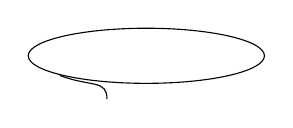
\begin{tikzpicture}\draw (0,0) ellipse (1.5 and .35);\draw (-1.1,-.25)..controls(-.7,-.4)and(-.5,-.3)..(-.5,-.55);\end{tikzpicture}} le foncteur $f_X^*:X_{\text{ét}}\mathbin{-}X_{\text{ét}}$ est \uline{isomorphe} au foncteur identique, d'où résulte que le morphisme \inserted{de Topos} qu'il induit $\unsure{F_X^*|f_X^*}:\widetilde X_{\text{ét}}\mathbin{-}\widetilde X_{\text{ét}}$ est une équivalence, isomorphe au foncteur identique \deleted{\unsure{par}}, par un isom \uline{unique} \uline{prolongeant} l'isomorphisme donné $F_{-/X}$ sur les faisceaux représentés. Donc b) $\Rightarrow$ a).
\mspage{33}
